\chapter{Results and Discussion}

\section{Ordinary MSD}



The results for the \gls{msd} in the ordinary case found in Eq. \ref{balpoint} can are summarized in Fig. \ref{fig:resultsMSDordinary} (taken from \cite{bothe}).

\begin{figure}[h!]
\begin{center}
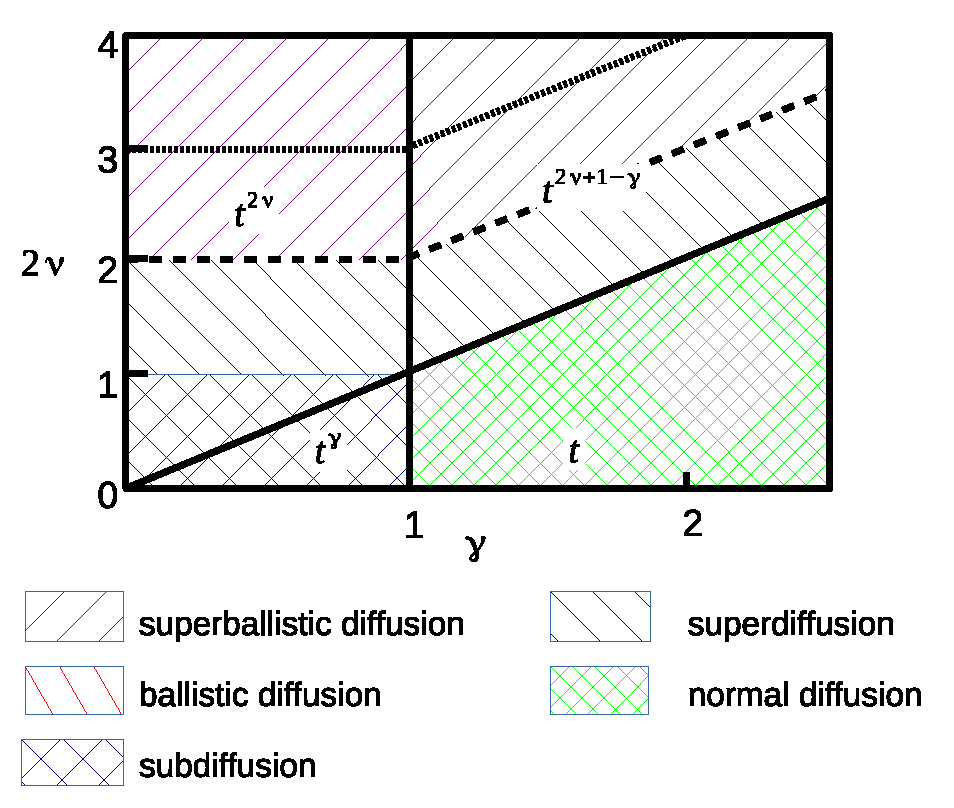
\includegraphics[width=90mm]{pics/resultsMSDordinary.eps}
\caption{The picture shows the asymptotic time dependence of the ensemble average $\langle x^2 \rangle \propto t^{x}$ in the ordinary L\'evy walk. The thick solid lines correspond to the changes in time exponent while the hatchings indicate the type of diffusion. The dashed line corresponds to ballistic behavior and the dotted one to the Richardson law.
\label{fig:resultsMSDordinary} }
\end{center}
\end{figure} 

We see that sub- as well as superdiffusion are realized in the ordinary case and that we can even reach superballistic diffusion for large values of $\eta$. This includes the Richardson regime, which is achieved for $\nu = 3/2$ for $\gamma <1$, and for $\nu = (\gamma + 2)/2$ for $\gamma > 1$. Also note that the area of normal diffusion is confined to the parameter ranges of $\gamma>1$, $2\nu < \gamma$. This corresponds to finite step duration and mean squared step length, which means the asymptotic \gls{PDF} is subject to the central limit theorem. We therefore expected normal diffusion in this region, which is confirmed by the results shown here.

We also see that the new parameter $\eta$ does not affect the time dependence, as it only affects the prefactor in leading order. Instead it governs the divergence that arises when calculating the second marginal moment of the distribution of incomplete steps, $r_2(t)$. Here we rederive the condition of convergence found in \cite{radons2018}, $\gamma > 2(\nu - \eta)$, which in the picture corresponds to the area below a diagonal line parallel to the bold one whose offset is given by $2\eta$. Increasing $\eta$ therefore increases the area of finite MSD in the picture, with $\nu=\eta$ always resulting in a finite MSD (since $\gamma >0$). From this we can see that for the original model with $\eta =1$ the Richardson regime for is either over or exactly on the line and therefore divergent. 

These results where tested through simulation, with an ensemble of $10^5$ particles. To ensure that the particles had time to reach the asymptotic behavior of $t>>t_0$ the last observation time was set to $t_{max} = 20000$
\footnote{All times are multiples of $t_0$, which was set to 1 in the simulation. Similarly all lengths are multiples of $c t_0^{\nu}$, which is also set to 1. }
I have then fitted the simulation results with $f(x) = a \; x^b$, with $b$ being the time exponent from the analytical calculations. We see in Fig. \ref{fig:plotMSDordinary} that the \gls{msd} indeed follows a power law, with the time exponent being in good agreement with the analytic predictions. This was tested further with simulations run with various configurations of $\gamma$, $\nu$ and $\eta$ and the  deviation from the predicted exponent was always smaller than 0.04. These small deviation can be explained by the influence of subleading terms for finite $t_{max}$. The simulation therefore confirms the results of the analytical calculation.
%
\begin{figure}
\begin{center}
\includegraphics[width=120mm]{pics/plotMSDordinary.png}
\caption{Time dependence of the ordinary MSD. The data was fitted with $f(x) = ax^b$.
\label{fig:plotMSDordinary} }
\end{center}
\end{figure} 
%

\todo{analyze regions of behavior along the lines of where step length and step variance diverge}

\section{Aged MSD}

For short aging times we reproduce the behavior of the ordinary walk in leading order up to prefactors, which is to be expected as the ordinary and aged results should coincide in the limit of $t_a \to 0$. We also find that in addition to $\gls{rest}_2(t)$ there is now a second possibly divergent contribution from $\gls{single}_2(t)$, but both have the same condition of convergence as the ordinary case, $\gamma > 2(\nu-\eta)$. 

For long aging times the region is the same, but the behavior of the walker differs significantly, which is illustrated in Fig. \ref{fig:resultsMSDaged} (taken from \cite{bothe}). 
%
\begin{figure}[h!]
\begin{center}
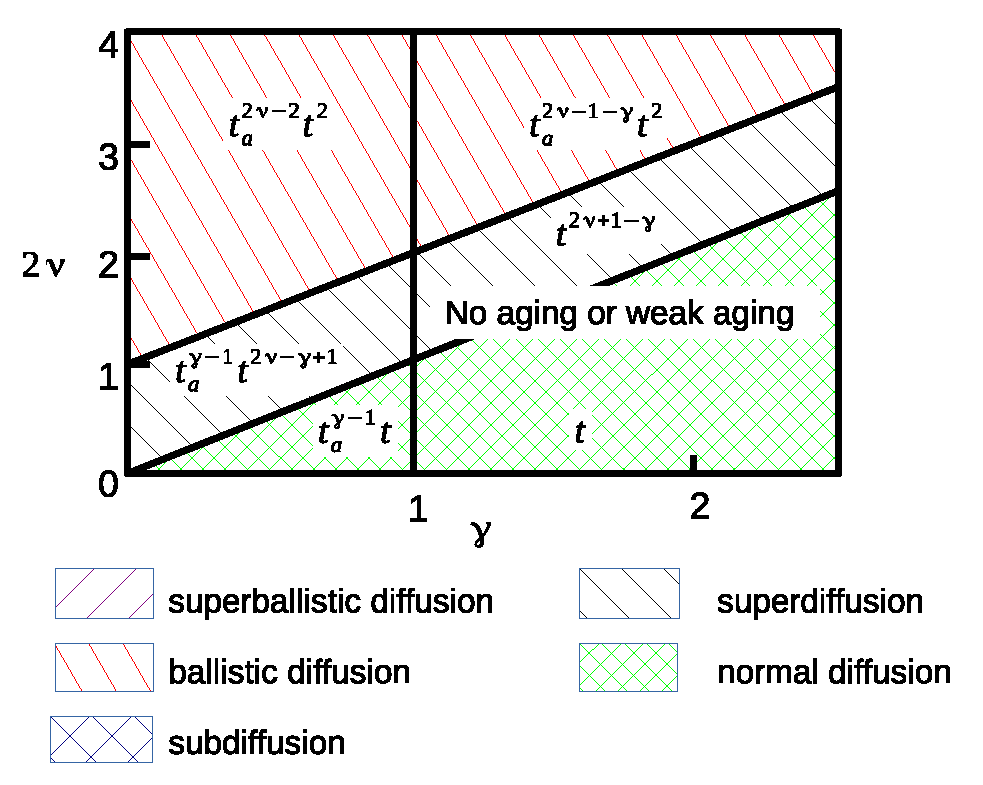
\includegraphics[width=90mm]{pics/resultsMSDaged.eps}
\caption{The panel shows the behavior of the ensemble average $\langle x^2(t) \rangle$ for the L\'evy walk in the limit of long aging times. The thick solid lines correspond to the changes in time-dependences while the hatchings represent the type of diffusion. The dashed line corresponds to the ballistic behavior, and the dotted one to the Richardson law.
\label{fig:resultsMSDaged} }
\end{center}
\end{figure} 
%
We see that for the parameter range where the ordinary walk showed subdiffusion we now find regular diffusion but with a prefactor that decays with growing aging times. There is no longer any superballistic diffusion and thus also no Richardson regime. However this does not make the model unsuitable for the description of the Richardson regime, since that relates to measuring the distance between two tracers immediately after they have been released into a stationary flow, i.e. corresponds to the ordinary case.\\ Furthermore we see that the aging leaves the parameter region with finite mean step duration ($\gamma<1$) unchanged wherever the ordinary walk showed normal or superdiffusive behavior ($2\nu < \gamma +1$).\\
The results for convergence are similar to the previous cases in that the second moment only exists for $\gamma>2(\nu-\eta)$, and if it exists the value of $\eta$ only enters the prefactors, but does not change the asymptotic power law dependences of the MSD, similar to the ordinary case.

It is noteworthy that the highest possible time exponent in the aged walk is quadratic, which seems counterintuitive since for small $\gamma$ long aging times correspond to an ensemble that is dominated by steps whose duration is much longer than the observation time and whose contribution to the \gls{msd} should scale strongly with time for large $\nu$. However this does not mean that the walkers move "slower" in the aged case but rather a result of the first order approximation in the observation time: Consider a walker whose step begins long before the beginning of observation at $-t_a$ and continues until the end of observation at $t$. His squared displacement during the observation is given by
%
\begin{align}
|x|^2 =& [c (t_a+t)^{\nu} - c (t_a+t)^{\nu-\eta} (t_a)^{\eta} ]^2\\
\simeq & c^2 \eta^2  (t_a+t)^{2\nu-2\eta} t_a^{2 \eta -2} t^2 \\
\simeq & c^2 \eta^2 t_a^{2 \nu -2} t^2 ,
\end{align}
%
which is exactly the result we see found for the parameter $\gamma <1$ and $2\nu > \gamma+1$ where such contributions dominate. The high speed of these cases is now shifted from the $t$ dependence to the prefactor which scales with $t_a$, similar to the way previously subdiffusive parameter ranges have now a prefactor that shrinks with larger aging times.

We moreover note that the double time-ensemble average $\langle \langle x^2 (t) \rangle_T \rangle_E$, also discussed in Ref. \cite{radons2018}, whose calculation involves an additional integration over the time,$\langle \langle x^2 (t) \rangle_T \rangle_E \simeq (T-t)^{-1} \int_0^{T-t} \langle x^2 (t|t_a) \rangle dt_a$  shows the same behavior as the aged walk if the measurement time $t$ is associated with the time lag in the double average, and the aging time $t_a$ is changed for the data acquisition time $T$.   

The verification via the simulation now involved the fitting of the MSD with regards to the observation as well as the aging time. The former was done analogously to the previous section and showed good agreement. For the aged time however considerable longer times where need, as both $t>> t_0$ and $t_a>> t$ had to be satisfied to reach the asymptotic limit. For an ensemble of $10^5$ walkers with $t_{max}=5\; 10^{3}$ and $t_{a,max} = 10^{6}$ the aging time exponent is in good agreement with  the analytical prediction as can be seen in Fig. \ref{fig:plotMSDaged}.
%
\begin{figure}
\begin{center}
\includegraphics[width=120mm]{pics/plotMSDaged}
\caption{Aging time dependence of the aged MSD. The data was fitted with $f(x) = ax^b$.
\label{fig:plotMSDaged} }
\end{center}
\end{figure} 
%
The analytical results have again been tested for various configurations of $\gamma$, $\eta$ and $\nu$ with the highest deviation of the aging time exponent from the analytic result being 0.06, which again is caused by the computational limits of reaching the asymptotic regime.


\section{Simulation of the ordinary PDF} \label{sec:simulatedPDF}

The \gls{PDF} was investigated numerically in one dimension by accumulating histograms for large ensembles of $10^{9}$ walkers. Since the \gls{PDF} is symmetric only the positive side is shown in the following figures.
%
\begin{figure}[H] % to enforce that it doesn't become a p float, which takes up the whole page
\begin{center}
\includegraphics[width=1\textwidth]{../CUDA_Simulation_RW/Results/Histograms/{histogram_gamma_0.6_nu_1.3_eta_1.3_ta_0}.png}
\caption{Histograms of a L\'evy walk with $\gamma =0.6$, $\nu = 1.3$ and $\eta =1.3$ at different points in time. The dashed line indicates the position a walker would have reached in a single step beginning at $t=0$ and ending exactly at the time of the respective panel.
\label{fig:histogramShapeEtaEqual} }
\end{center}
\end{figure} 
%
Unlike the \gls{msd}, where the new parameter $\eta$ only changes the prefactors of finite results,  $\eta$ has a major impact on the shape of the \gls{PDF}: \\
In the case $\nu=\eta$ shown in Fig. \ref{fig:histogramShapeEtaEqual} the histogram has a clear cutoff marked by a delta peak with a continuous left flank that coincides with the position a walker can reach in a single step of duration $t$. This is similar to what you find for the similar velocity model ($\eta=\nu=1$), \todo{source} where the \gls{PDF} also has a clear boundary after which no walker can be found. \\
This can be understood by considering the displacement in the first step of a walk,
%
\begin{align}
\abs{\ve{x}_{n+1}} = c \gls{dur}_{1}^{\nu-\eta} t^{\eta} , \label{eqn:step}
\end{align}
% 
where we recall that $\gls{dur}_{1}$ is the total duration of the step, which may be longer than the observation time $t$. In the case of $\eta=\nu$ the dependence on the total step duration vanishes, which means that any particle starting at $t=0$ moves with the same speed, regardless of how long the step will last. Since $\eta>1$ the greatest displacement is archived when the particle performs a single step whose duration is greater or equal than the observation times. This means two things: Firstly, no particle can be found beyond this limit and secondly, the entire probability of having a step duration of $t$ or longer is concentrated on this particular cutoff, which corresponds to a delta peak in the probability density, which explains that feature of the histograms. \\
For the rest of the \gls{PDF} we see the highest probability besides the peak at the origin, which is consistent with it being a isotropic model, and then the density decays exponentially with the distance from the origin, $\gls{pdf} \propto e^{-|x|}$. Directly before the peak a minor notch can be seen in the histogram, whose origin is unclear.  \\
%
\begin{figure}[H] % to enforce that it doesn't become a p float, which takes up the whole page
\begin{center}
\includegraphics[width=1\textwidth]{../CUDA_Simulation_RW/Results/Histograms/{histogram_gamma_0.6_nu_1.3_eta_1.1_ta_0}.png}
\caption{Histograms of a L\'evy walk with $\gamma =0.6$, $\nu = 1.3$ and $\eta =1.1$ at different points in time. The dashed line indicates the position a walker would have reached in a single step beginning at $t=0$ and ending exactly at the time of the respective panel.
\label{fig:histogramShapeEtaSmall} }
\end{center}
\end{figure} 
%
However this shape of the \gls{PDF} changes profoundly when modifying $\eta$, as can be seen in Fig \ref{fig:histogramShapeEtaSmall}: Here both $\gamma$  and $\nu$ are identical to the previous picture but $\eta$ is now smaller than $\nu$. Now walkers travel well beyond the limit of what can be reached in a single step of total duration $t$ and there is no longer a  delta peak. Instead the dashed line marks the distinction between a simple exponential decay close to the origin and a faster decay further away. \\
This shape can again be understood when considering Eq. (\ref{eqn:step}): Since $\eta < \nu$ the observation time independent prefactor of the displacement now grows with the total step duration. This means that walkers whose step duration is larger than the observation time can reach arbitrarily high initial velocities and therefore move well beyond the dashed line. Consequently the walker has a finite probability to be at any point for $t>0$, which is not fully captured here since the histogram only covers a finite range and the positions of walkers that move beyond the histogram range cannot be shown. \\
Also note that while very long steps are not extremely rare (the mean step duration diverges in the case $\gamma >1$) for finite ensembles these outliers are nevertheless hard to capture and even for $10^{9}$ walkers we see the limits of the simulation in the edges of the \gls{PDF}, where it becomes discontinuous. 
%
\begin{figure}[H] % to enforce that it doesn't become a p float, which takes up the whole page
\begin{center}
\includegraphics[width=1\textwidth]{../CUDA_Simulation_RW/Results/Histograms/{histogram_gamma_0.6_nu_1.3_eta_1.5_ta_0}.png}
\caption{Histograms of a L\'evy walk with $\gamma =0.6$, $\nu = 1.3$ and $\eta =1.5$ at different points in time. The dashed line indicates the position a walker would have reached in a single step beginning at $t=0$ and ending exactly at the time of the respective panel.
\label{fig:histogramShapeEtaLarge} }
\end{center}
\end{figure} 

Moving on to the case of $\eta> \nu$ as shown in Fig. \ref{fig:histogramShapeEtaLarge} we see that the shape of the \gls{PDF} is again very different: Similar to the $\eta = \nu$ case the dashed line marks a clear limit of how far a walker can reach, but there is no delta peak. Inspecting Eq. (\ref{eqn:step}) again we see the reason: Because we have $\eta> \nu$ the prefactor in the displacement actually grows smaller with increasing total step duration, meaning that any walker performing a step with duration longer than $t$ can actually not reach the limit, meaning that only walkers with a step duration of exactly $t$ can reach the cutoff, the probability of which is infinitesimal. 

These findings explain the convergence condition we rederived for the \gls{msd}, $\gamma > 2(\nu-\eta)$: For $\eta \geq \nu$ the support of the \gls{PDF} is bounded and therefore the \gls{msd} always converges. For $\eta < \nu$ this is no longer the case and there is a finite probability to find the walker at any distance from the origin for $t>0$. Convergence now depends on the likelihood of extreme events, meaning that $\gamma$ has to be sufficiently large for the \gls{msd} to exist.
%
\begin{figure}[H] % to enforce that it doesn't become a p float, which takes up the whole page
\begin{center}
\includegraphics[width=1\textwidth]{../CUDA_Simulation_RW/Results/Histograms/{histogram_gamma_0.6_nu_0.8_eta_0.8_ta_0}.png}
\caption{Histograms of a L\'evy walk with $\gamma =0.6$, $\nu = 0.8$ and $\eta =0.8$ at different points in time. The dashed line indicates the position a walker would have reached in a single step beginning at $t=0$ and ending exactly at the time of the respective panel.
\label{fig:histogramShapeNuSmall} }
\end{center}
\end{figure} 

Next we are interested in the influence of the parameter $\nu$ on the shape of the \gls{PDF}, which is illustrated in Fig. \ref{fig:histogramShapeNuSmall}: We are again in the case of $\eta = \nu$, but unlike in Fig. \ref{fig:histogramShapeEtaEqual} the dashed line no longer marks a sharp boundary of the \gls{PDF} and there is a finite probability for a walker to be found beyond it. However this is not due to steps with durations longer than the observation time (all these cases reach exactly the boundary and contribute to the peak) but instead due to walkers that take more than one step: Since $\nu<1$ the maximum displacement is not realized by making a single long step, but rather by taking many smaller steps in the same direction, simply because the sum of a root is larger than the root of a sum. It follows that values of $\nu<1$ cause the breakdown of the sharp cutoff and the simulations show that this effect becomes more impactful with smaller $\eta$. {\color{red} However this does not cause divergence of the \gls{msd} because so many steps are almost never realized for power law step duration distributions.  }

\begin{figure}[H] % to enforce that it doesn't become a p float, which takes up the whole page
\begin{center}
\includegraphics[width=1\textwidth]{../CUDA_Simulation_RW/Results/Histograms/{histogram_gamma_1.2_nu_1.3_eta_1.3_ta_0}.png}
\caption{Histograms of a L\'evy walk with $\gamma =1.2$, $\nu = 1.3$ and $\eta =1.3$ at different points in time. The dashed line indicates the position a walker would have reached in a single step beginning at $t=0$ and ending exactly at the time of the respective panel.
\label{fig:histogramShapeGammaLarge} }
\end{center}
\end{figure} 
%
Furthermore we consider the effect of varying $\gamma$ on the \gls{PDF} which is shown in in Fig. \ref{fig:histogramShapeGammaLarge}. Comparing this to Fig. \ref{fig:histogramShapeEtaEqual}, which differs only in its $\gamma$ value, we see that the peak is much less prominent but the position of the cutoff doesn't change. Furthermore we see that the \gls{PDF} is much more centered on the origin . This makes sense as a larger value of $\gamma$ makes steps longer than the observation time much more unlikely and the walk is therefore less dominated by these extreme events, which would be contributing to the height of the delta peak.

Finally we are interested in the case where both the mean step duration as well as the variance of the step length exist ($\gamma>1$, $\gamma > 2\nu$). As can be seen in Fig. \ref{fig:histogramGauss} 
%
\begin{figure}[H] % to enforce that it doesn't become a p float, which takes up the whole page
\begin{center}
\includegraphics[width=1\textwidth]{../CUDA_Simulation_RW/Results/Histograms/{histogram_gamma_1.2_nu_0.4_eta_0.4_ta_0}.png}
\caption{Histograms of a L\'evy walk with $\gamma =1.2$, $\nu = 0.4$ and $\eta =0.4$ at different points in time. The dashed line indicates the position a walker would have reached in a single step beginning at $t=0$ and ending exactly at the time of the respective panel.
\label{fig:histogramGauss} }
\end{center}
\end{figure}
%
the \gls{PDF} takes the form of a Gaussian in this regime as is predicted by the central limit theorem. The Gaussian is not bounded by a single step displacement because $\nu<1$ holds as explains above. Unlike the previous cases this result is independent of the value of $\eta$.

\section{Simulation of the aged PDF}

The \gls{PDF} of the generalized L\'evy walk changes considerably under aging. An example of this is for the case $\nu=\eta$ shown in Fig. \ref{fig:histogramAgedEtaEqual}
%
\begin{figure}[H] 
\begin{center}
\includegraphics[width=1\textwidth]{../CUDA_Simulation_RW/Results/Histogram_aged/{histogram_gamma_0.6_nu_1.3_eta_1.3_ta_1e+05}.png}
\caption{Histograms of an aged  L\'evy walk with $\gamma =0.6$, $\nu = 1.3$ and $\eta =1.3$ and aging time $t_a = 10^{5}$ at different points in time. The dashed line indicates the position a walker would have reached in a single step beginning at $t=0$ and ending exactly at the time of the respective panel. The dotted line indicates the displacement a step could archive during the observation if it starts at $-t_a$ and ends at $t$.
\label{fig:histogramAgedEtaEqual} }
\end{center}
\end{figure}
%
where we can observe two jumps in the \gls{PDF}, as opposed to one in the ordinary case, which correspond to two different events: The red line denotes the distance covered by a jump starting at the beginning of observation end ending precisely at $t$, the second, yellow line corresponds to walkers that started their step at $-t_a$ and end it at $t$. \\
Left of the dashed red line the probability is small, as this area captures only events that had a change time since the beginning of observation, which is exceedingly rare for growing $t_a$, because the walker getting locked into longer and longer steps. 
{\color{blue} 
However it is unclear why there is a notch exactly at the red line, since we don't expect a step ending at the beginning of observation to be more likely than at any other time.
}
All events beyond the red line correspond to steps that started before the beginning of observation with the upper limit given by a step starting at $-t_a$, which is indicated by the green line. Similar to the ordinary case we see a delta peak with a left flank here. This peak captures the probability of all cases that started at $-t_a$ and whose total step duration is equal or longer than $t_a+t$. Also note that the probability to find the particle at the origin is actually pretty small compared to the peak at maximum displacement. This is again caused by the large number of particles that are already locked into long steps at the beginning of observation.\\

Varying $\eta$ has an effect on the aged \gls{PDF} that is very similar to that in the ordinary case: For $\eta > \nu$ the peak vanishes and the probability to reach the second line becomes infinitesimal and for $\eta < \nu$ the yellow line no longer restricts the \gls{PDF} as the walker can now reach arbitrary distances. 

However something interesting happens when we enter the regime $\nu<1$, which is depicted in Fig. \ref{fig:histogramAgedEtaEqual}.
%
\begin{figure}[H] 
\begin{center}
\includegraphics[width=1\textwidth]{../CUDA_Simulation_RW/Results/Histogram_aged/{histogram_gamma_0.6_nu_0.8_eta_0.8_ta_1e+05}.png}
\caption{Histograms of an aged  L\'evy walk with $\gamma =0.6$, $\nu = 0.8$ and $\eta =0.8$ and aging time $t_a = 10^{5}$ at different points in time. The dashed line indicates the position a walker would have reached in a single step beginning at $t=0$ and ending exactly at the time of the respective panel. The yellow line indicates the displacement a step could archive during the observation if it starts at $-t_a$ and ends at $t$.
\label{fig:histogramAgedNuSmall} }
\end{center}
\end{figure}
%
We see that the yellow line is closer to the origin than the red one, the reason for this being that the longest step durations no longer correspond to the biggest displacements for $\nu < 1$. Directly at the yellow line the \gls{PDF} forms a peaks, due to the large number of walkers that have only performed one step so far. The flank of this peak is continuous on the right side, as these cases correspond to walkers that have also entered a very long step, but only slightly after the process began to age. Events left of the peak belong to walkers that reached a change point and changed directions, thus causing a smaller displacement from the origin. Further to the right we find the red dashed line, marking a sharper decrease in the flank of the \gls{PDF}. As in the ordinary case with $\nu<1$ walkers can move beyond this line by performing multiple steps in the same direction, but this gets exceedingly rare and the probability density falls of quickly.


\section{Probability density at the origin}

During the analytical approximation of the \gls{PDF} in Sec. \ref{sec:calcPDF} we derived a prediction for the time dependence of  the probability density at the origin, which is tested in the simulation. The results of the analytical calculation are shown in Fig. \ref{fig:resultsPDF}.
%
\begin{figure}[H] % to enforce that it doesn't become a p float, which takes up the whole page
\begin{center}
\includegraphics[width=0.8\textwidth]{pics/resultsPDF.png}
\caption{The time dependence of the probability density for different values of the parameters $\nu $ and $\gamma$ is shown. Thick lines indicate the distinction between two different regimes.
\label{fig:resultsPDF} }
\end{center}
\end{figure} 
%
By plotting the change in the \gls{PDF} at the origin over a period double logarithmically we can extract the time exponent, as is shown in Fig. \ref{fig:fitPDFOrigin}.
%
\begin{figure}[H] % to enforce that it doesn't become a p float, which takes up the whole page
\begin{center}
\includegraphics[width=0.8\textwidth]{../CUDA_Simulation_RW/Results/Histogram_origin_peak/{origin_peak_gamma_1.5_nu_0.8_eta_0.8}.png}
\caption{A fit of time dependence of the probability density for the parameter values $\gamma=1.5$, $\nu =0.8 $ and $\eta=0.8$ is shown in a doubly logarithmic plot.
\label{fig:fitPDFOrigin} }
\end{center}
\end{figure} 
%
We see that the \gls{PDF} is indeed of the form $t^{x}$ and the deviation of the time exponent from the expected result, $t^{-0.55}$, are small. Fits with various other parameters confirm this result, with deviations always being smaller than 0.02

\section{Analytic results for the PDF} \label{analyticResultsPDF}

We now turn our attention to the approximation for the \gls{PDF} derived in Sec. \ref{sec:calcPDF}. Through numerical evaluation of the inverse Laplace transform we obtained a semi-analytic result for the \gls{PDF} which in the case of $\alpha = 0.8$ is compared to the corresponding simulation in Fig. \ref{fig:inverseLaplaceI}.
%
\begin{figure}[H] % to enforce that it doesn't become a p float, which takes up the whole page
\begin{center}
\includegraphics[width=0.8\textwidth]{{../CUDA_Simulation_RW/Results/InverseLaplace/histogram_a_0.8_gamma_0.6_nu_0.8_eta_1_ta_0}.png}
\caption{Comparison of the histogram obtained in a simulation with $\gamma=0.6$, $\nu =0.8 $ and $\eta=1$ with the corresponding rescaled semi-analytic result for $\alpha=0.8$.
\label{fig:inverseLaplaceI} }
\end{center}
\end{figure} 
%
Since the prefactors of the semi-analytic result were lost in the calculation the length scale and overall height of the expression were rescaled to match that of the simulation. While the behavior for large displacements is somewhat similar we see that despite the rescaling the semi-analytic result is not in good agreement with the simulation, with the initial slope being very different. The contrast is even more stark when one considers different values of $\eta$, which we have seen to have a considerable influence on the shape of the \gls{PDF}  (see Fig. \ref{fig:histogramShapeNuSmall}) but don't impact the analytic expression. Comparisons with different values of $\alpha$, which are not shown here, give a similar result.

This is caused by the approximation made in the calculation, where $\gls{rest}$ and $\gls{psi}$ were expanded to second order, which we know from the calculation of the \gls{msd} does not depend on $\eta$ in the asymptotic limit. This is fine for the \gls{msd}, whose time exponent is indeed independent of $\eta$. but for the \gls{PDF} this approach misses much of the rich behavior seen in Sec. \ref{sec:simulatedPDF}.  

However the approximation is not completely off: As we have seen in the previous section the prediction for the time dependence of the \gls{PDF} at the origin is accurate and  it also correctly predicts the parameter region where the \gls{PDF} tends to a Gaussian, which corresponds to $\alpha = 1/2$ (see Fig. \ref{fig:alphaValuesPDF}). Here the simulated \gls{PDF} loses its dependence on $\eta$ and the two results match, as is depicted in Fig. \ref{fig:inverseLaplaceGauss}.
%
\begin{figure}[H] % to enforce that it doesn't become a p float, which takes up the whole page
\begin{center}
\includegraphics[width=0.8\textwidth]{{../CUDA_Simulation_RW/Results/InverseLaplace/histogram_a_0.5_gamma_1.2_nu_0.4_eta_0.4_ta_0}.png}
\caption{Comparison of the histogram obtained in a simulation with $\gamma=1.2$, $\nu =0.4$ and $\eta=0.4$ with the corresponding rescaled analytic result for $\alpha=0.5$.
\label{fig:inverseLaplaceGauss} }
\end{center}
\end{figure} 